\section{Comparação entre os Avanços da Implementação}

\subsection{Axial e mais gdl}
\begin{figure}[H]
	\centering
	\caption{Force}
	\label{fig:Force}
	
	\begin{minipage}{0.7\textwidth}
		\centering
		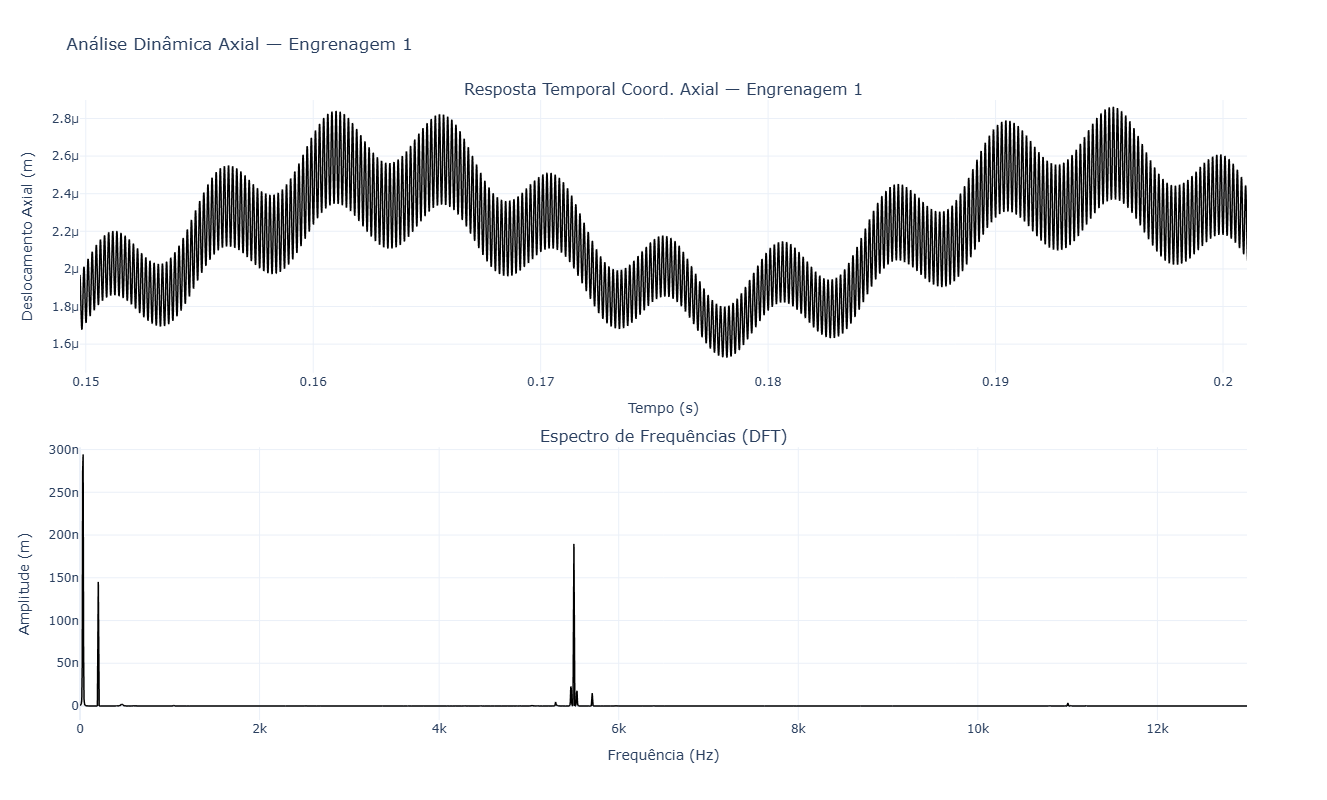
\includegraphics[width=\linewidth]{results/replan_axial.png}
		\par\vspace{0.3em}
		\raggedright
		{\small Fonte: Elaborado pelo autor.}
	\end{minipage}
\end{figure}

\subsection{suavização}

\begin{table}[H]
	\centering
	\begin{threeparttable}
		\caption{Comparação dos parâmetros e resultados das simulações}
		\label{tab:comparacao_simulacoes}
		
		\begin{tabular}{lcc}
			\hline
			Parâmetro/Dado & Simulação 1 & Simulação 2 \\
			\hline
			Suavização ativada & Sim & Não \\
			Valor de $\sigma$ da suavização & -- & -- \\
			Passo de tempo & -- & -- \\
			Ciclos simulados & -- & -- \\
			Tempo de simulação total & -- & -- \\
			\hline
		\end{tabular}
		
		\begin{tablenotes}[para, flushleft]
			\small
			\item Fonte: Elaborado pelo autor.
		\end{tablenotes}
		
	\end{threeparttable}
\end{table}

\begin{figure}[H]
	\centering
	\caption{Bifurcation}
	\label{subfigure}
	
	\begin{minipage}{\textwidth}
		\centering
		
		\begin{subfigure}{\textwidth}
			\centering
			\caption{no smooth}
			\label{subfig:Bifurcation}
			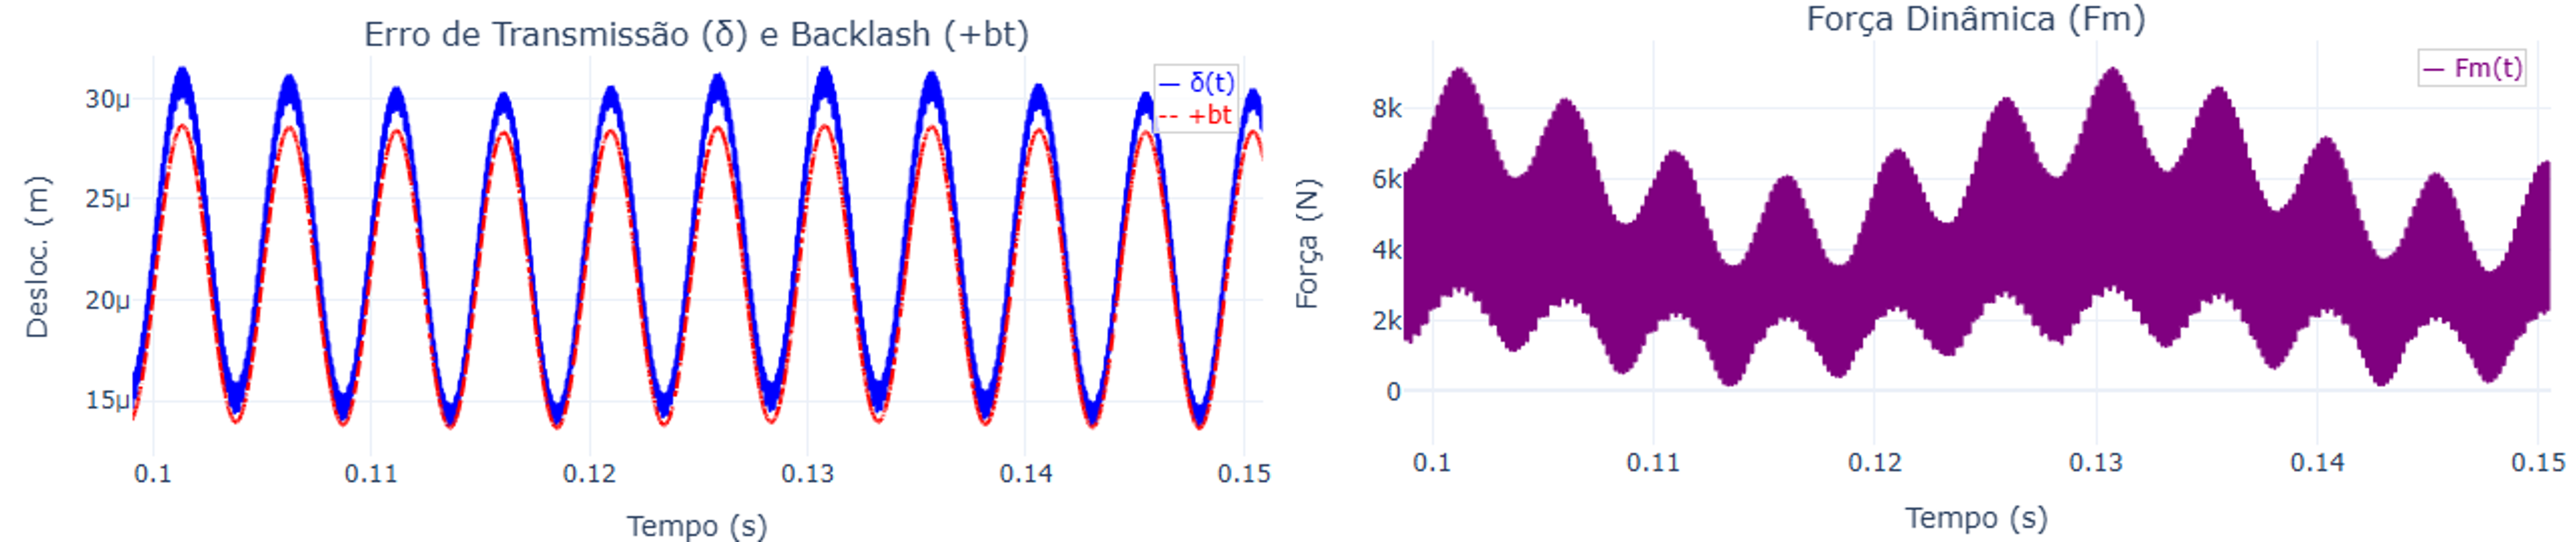
\includegraphics[width=\linewidth]{results/replan_no_smooth.png}
		\end{subfigure}
		\hspace{10pt} \\
		\begin{subfigure}{\textwidth}
			\centering
			\caption{smooth}
			\label{subfig:Bifurcation}
			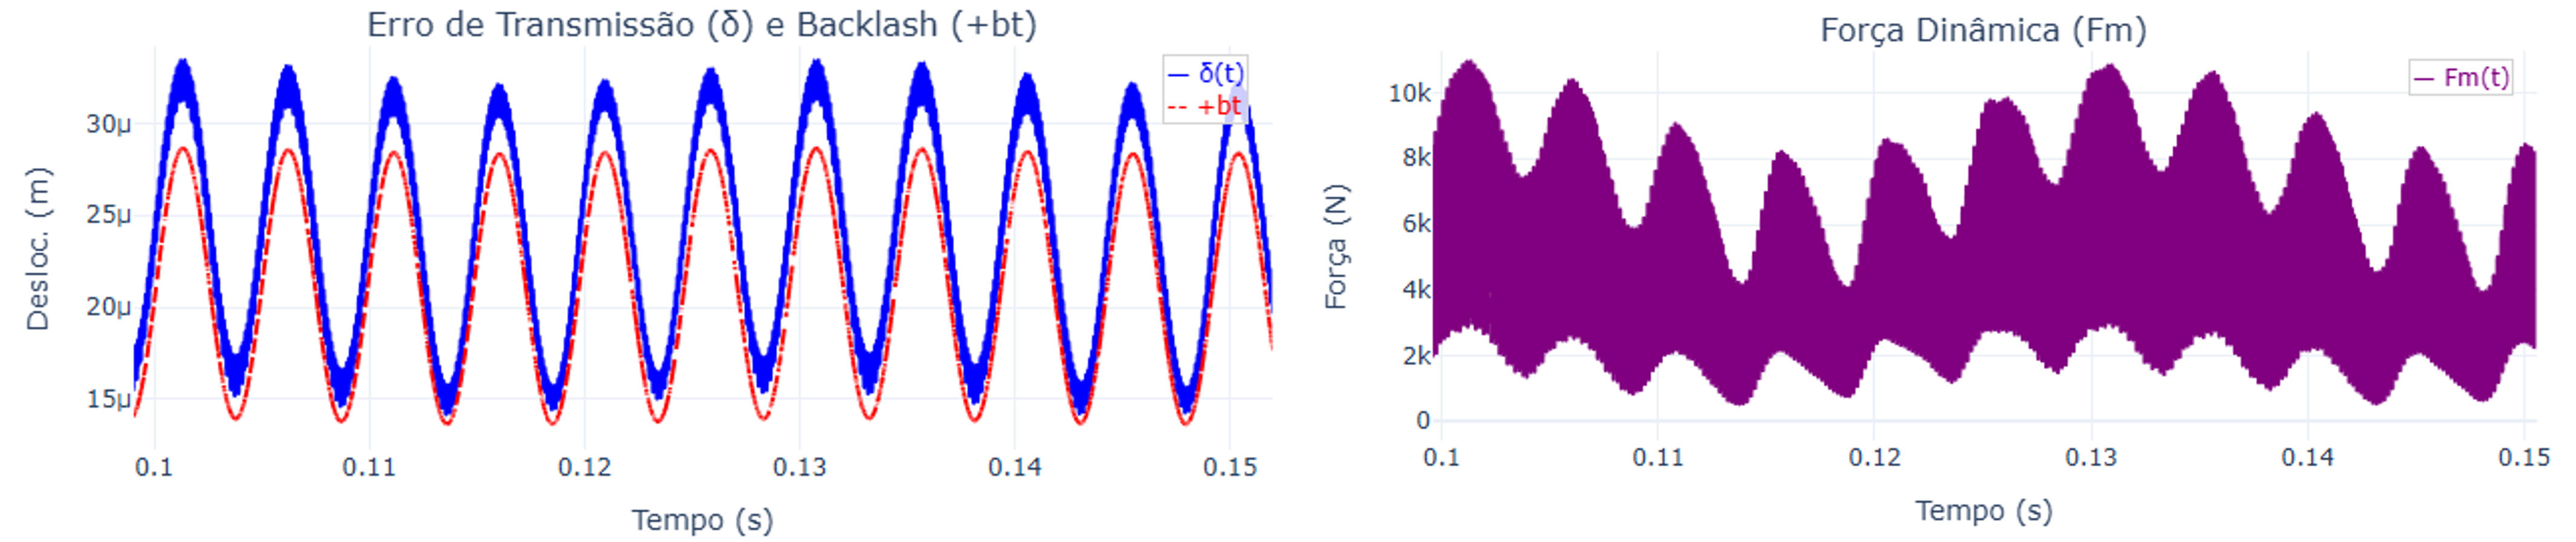
\includegraphics[width=\linewidth]{results/replan_smooth.png}
		\end{subfigure}
		
		\par\vspace{0.5em}
		\raggedright
		{\small Fonte: Elaborado pelo autor.}
	\end{minipage}
\end{figure}
